\section{Подготовительные действия}

Для организации виртуального пространства, в первую очередь необходимо установить операционную систему на хост-компьютер. 
В качестве хост-компьютера может выступать как сервер, так и настольный компьютер.

В данном руководстве описывается установка и настройка ОС CentOS 6\footnote{Образы для скачивания: \url{http://mirror.yandex.ru/centos/6.6/isos/}}.
CentOS основан на коммерческом дистрибутиве Red Hat Enterprise Linux (RHEL). 
RHEL состоит из свободного ПО с открытым кодом, однако доступен в виде дисков с бинарными пакетами только для платных подписчиков. 
Red Hat предоставляют исходные коды системы, так как это предполагается лицензией GNU/GPL.
Разработчики CentOS используют данный исходный код для создания окончательного продукта, очень близкого к RHEL и доступного для скачивания.
Срок поддержки CentOS "--- десять лет.

\subsection{Установка и настройка CentOS}
Программа установки CentOS проста в использовании и локализована почти на все языки мира. 
В качестве системного, рекомендуется использовать язык по умолчанию (english).

Во время установки, помимо выбора языка необходимо указать пароль суперпользователя (root), например \texttt{p@ssw0rd} и имя узла, например \texttt{centos.openvz}.

На жестком диске нужно создать как минимум 3 раздела:
\begin{itemize}
\item \texttt{/} "--- не менее 6G (ext4) "--- корневой раздел;
\item \texttt{swap} "--- 1G\footnote{Размер swap должен быть равен примерно половине объема оперативной памяти} "--- раздел подкачки;
\item \texttt{/vz} "--- все остальное дисковое пространство (ext4).
\end{itemize}

Пошаговая установка CentOS 6 описана в прил. \ref{pril:a}.

После установки ОС, необходимо перезагрузиться.

Первый вход в систему осуществляется с учетной записи суперпользователя. Логин "--- \texttt{root}, пароль\footnote{Во время ввода пароля, число его символов не отображается, это сделано в целях безопасности} "--- \texttt{p@ssw0rd}.

После входа в систему, пользователю будет доступен консольный интерфейс интерпретатора командной строки (bash). 
С помощью ввода команд в интерпретаторе, осуществляется работа в ОС GNU/Linux.
\clearpage
Строка ввода команд выглядит примерно так:
\begin{lstlisting}
[root@centos ~]# 
\end{lstlisting}
где:
\begin{itemize}
    \item \texttt{root} "--- имя текущего пользователя;
    \item \texttt{centos} "--- имя компьютера (задавали при установке);
    \item \texttt{\~} "--- {текущий каталог}\footnote{Для просмотра имени текущего каталога используется команда \texttt{pwd}}, в котором находится пользователь.
\end{itemize}

Символ \texttt{\#} означает, что в данный момент вход осуществлен пользователем \texttt{root}.

Для безопасной работы с GNU/Linux нужно иметь как минимум одного локального пользователя отличного от \texttt{root}.
Пусть этим пользователем будет \texttt{stud} c паролем \texttt{\$tud}:
\begin{lstlisting}
# adduser stud
# passwd stud
New password: $tud
\end{lstlisting}

Теперь, во время входа в систему, можно указать пользователя \texttt{stud} и пароль \texttt{\$tud}:
\begin{lstlisting}
# exit
centos login: stud
Password: $tud
Last login: Mon Jan 01 12:12:12 on tty1
[stud@centos ~]$ 
\end{lstlisting}

Чтобы переключиться в системе с пользователя \texttt{stud} на \texttt{root} можно выполнить команду:
\begin{lstlisting}
$ su -
Password: p@ssw0rd
[root@centos ~]#  
\end{lstlisting}

По умолчанию в CentOS после перезагрузки сетевые интерфейсы не включаются. 
Нужно сделать так, чтобы при загрузке системы интерфейсы поднимались сами:
\begin{lstlisting}
# vi /etc/sysconfig/network-scripts/ifcfg-eth0
ONBOOT="yes"
\end{lstlisting}
\begin{lstlisting}
# ifup eth0
\end{lstlisting}

\subsection{Обновление пакетной базы программ}
Для установки, удаления и обновления программ, в CentOS существует утилита \texttt{yum}. 
На сервере важно всегда обновлять программное обеспечение, так как в новых версиях не только могут добавлять новые возможности, но и исправлять уязвимости.
Указанная ниже команда обновляет все существующие в системе пакеты:
\begin{lstlisting}
# yum update
\end{lstlisting}

Для удобства работы в ОС рекомендуется установить следующее ПО:
\begin{itemize}
\item \texttt{vim} (текстовый редактор);
\item \texttt{wget} (утилита для скачивания файлов);
\item \texttt{nslookup} (утилита для работы с DNS);
\item \texttt{man}\footnote{Для того, чтобы узнать как правильно пользоваться командой \texttt{man} можно выполнить команду \texttt{man man}} (руководства к программам).
\end{itemize}

\begin{lstlisting}
# yum install vim wget bind-utils man
\end{lstlisting}

Чтобы установить \texttt{htop} (утилиту системного мониторинга), нужно подключить дополнительный репозиторий \texttt{rmpforge}:
\begin{lstlisting}
# cd /tmp
# wget http://pkgs.repoforge.org/rpmforge-release/rpmforge-release-0.5.3-1.el6.rf.x86_64.rpm
# rpm -Uhv rpmforge-release*.rf.x86_64.rpm
# yum install htop
\end{lstlisting}

\subsection{Настройка времени системы}
Для сервера очень важно, чтобы было установлено правильное время.

Чтобы синхронизировать время с интернетом необходимо установить пакет \texttt{ntp}:
\begin{lstlisting}
# yum install ntp
# service ntpd start
Starting ntpd:                                     [  OK  ]
# ntpdate -bs pool.ntp.org
# date
Mon Jan 01 12:12:12 MSK 2014
\end{lstlisting}

\subsection{Установка ядра и утилит OpenVZ}
Для установки ядра и утилит OpenVZ нужно добавить репозиторий и импортировать ключ:
\begin{lstlisting}
# wget -P /etc/yum.repos.d/ http://ftp.openvz.org/openvz.repo
# rpm --import http://ftp.openvz.org/RPM-GPG-Key-OpenVZ
\end{lstlisting}

Установка \texttt{vzkernel} (ядра OpenVZ):
\begin{lstlisting}
# yum install vzkernel
\end{lstlisting}

%Настраиваем параметры ядра\footnote{В \texttt{vzctl} версии 4.4 и выше, настройки параметров ядра не обязательны}, необходимые для работы OpenVZ:
%\begin{lstlisting}
%# vim /etc/sysctl.conf
%net.ipv4.ip_forward = 1
%net.ipv4.conf.default.proxy_arp = 0
%net.ipv6.conf.default.forwarding = 1
%net.ipv6.conf.all.forwarding = 1
%net.ipv4.conf.all.rp_filter = 1
%kernel.sysrq = 1
%net.ipv4.conf.default.send_redirects = 1
%net.ipv4.conf.all.send_redirects = 0
%\end{lstlisting}

%Отключаем \texttt{SELinux}\footnote{SELinux (англ. Security-Enhanced Linux) "--- реализация системы принудительного контроля доступа, которая может работать параллельно с классической избирательной системой контроля доступа}:
%\begin{lstlisting}
%# echo "SELINUX=disabled" > /etc/sysconfig/selinux
%\end{lstlisting}

Устанавливаем инструменты, необходимые для работы с OpenVZ:
\begin{lstlisting}
# yum install vzctl vzquota ploop
\end{lstlisting}

%По умолчанию в OpenVZ настроен IPTables который блокирует некоторые соединения.

%Очищаем все правила IPTables, оставив в файле строки:
%\begin{lstlisting}
%# vim /etc/sysconfig/iptables
%*filter
%:INPUT ACCEPT [0:0]
%:FORWARD ACCEPT [0:0]
%:OUTPUT ACCEPT [0:0]
%COMMIT
%\end{lstlisting}
%\begin{lstlisting}
% service iptables restart
%\end{lstlisting}

Для применения новых настроек нужно перезагрузиться:
\begin{lstlisting}
# reboot
\end{lstlisting}

Во время перезагрузки в меню загрузчика GRUB появится пункт \texttt{OpenVZ} (рис.~\ref{pic:grub}).
С этого ядра и нужно загружаться.
\begin{figure}[ht]
    \centering
	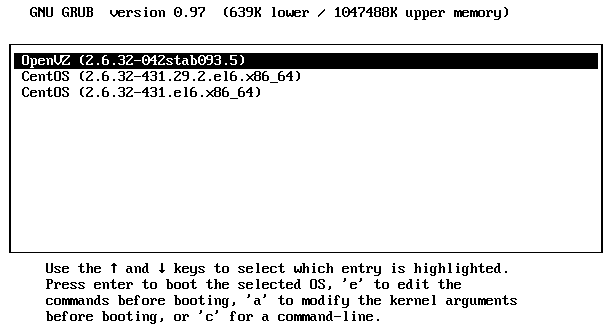
\includegraphics[width=0.8\linewidth]{grub.png}
	\caption{Меню загрузчика GRUB}\label{pic:grub}
\end{figure}

\subsection{Загрузка шаблонов для гостевых ОС}

На основе файлов шаблонов OpenVZ, будут работать гостевые операционные системы.

Полный список доступных для загрузки шаблонов\footnote{Шаблон "--- согласно определению, это ряд пакетов от некоторого распределения Linux, используемых для заселения VPS.
Шаблон ОС состоит из системных программ, библиотек, и скриптов, необходимых, так же как основные приложения и утилиты} можно посмотреть командой:
\begin{lstlisting}
# vztmpl-dl --list-all
\end{lstlisting}

Загрузим шаблоны для Debian, Ubuntu, CentOS и openSUSE:
\begin{lstlisting}
# vztmpl-dl debian-7.0-x86_64-minimal \
> ubuntu-14.04-x86_64-minimal \
> centos-7-x86_64-minimal \
> suse-13.1-x86_64-minimal \
> centos-6-x86_64-minimal \
> 
\end{lstlisting}

\clearpage
